% !TEX root = ../main.tex
\chapter{Related Work} \label{ch:reated_work}

In this chapter, we give an overview of graph based algorithms
for image segmentation 

\section{Multicut}\label{sec:rw_multicut}

Segmentation is an important problem in computer vision as a first step
towards understanding an image. Many algorithms start with an over-segmentation
into superpixels, which are then clustered into ``perceptually meaningful''
regions.
Usually, the number of these regions is not known beforehand.

Recently, the multicut formulation~\cite{chopra_1993_mp}
(sometimes called \emph{correlation clustering}, \cite{bansal_2004_ml})
has become increasingly popular for unsupervised
image segmentation.
Given an edge-weighted region adjacency graph,
the problem is to find the segmentation which
minimizes the cost of the cut edges.
Such an approach has been shown to yield
state-of-the-art results on the Berkeley Segmentation Database
%TODO: - alush_2013_simbad apply it on BSD500, is is state-of-the-art?
%      - gPb-owt is not really learned? Do we need to say this????
\cite{andres_2011_iccv,yarkony_2012_eccv,alush_2013_simbad}.


In this section we will motivate the multicuts and show the basic problem formulation.
In \cref{ch:cgc} we will give an more detailed overview of different solvers
for the multicut objective and introduce a new approximative solver. 


\section{Hierarchical Clustering}\label{sec:rw_hc}


\begin{tikzpicture}[scale=  1,every node/.style={minimum size=1cm},on grid]
        
    %slanting: production of a set of n 'laminae' to be piled up. N=number of grids.
    

    %%%%%%%%%%%%%%%%%%%%%%%%%%%%%%%%%%%%%%%%%%%%%%%%%%%%%%%%%%%%%%%
    % 0 bottom layer
    %%%%%%%%%%%%%%%%%%%%%%%%%%%%%%%%%%%%%%%%%%%%%%%%%%%%%%%%%%%%%%%%
        
    \begin{scope}[yshift=0,every node/.append style={yslant=0.5,xslant=-1},yslant=0.5,xslant=-1]
        \draw[-latex,thick] (-0.17,3.21/2) node[right]{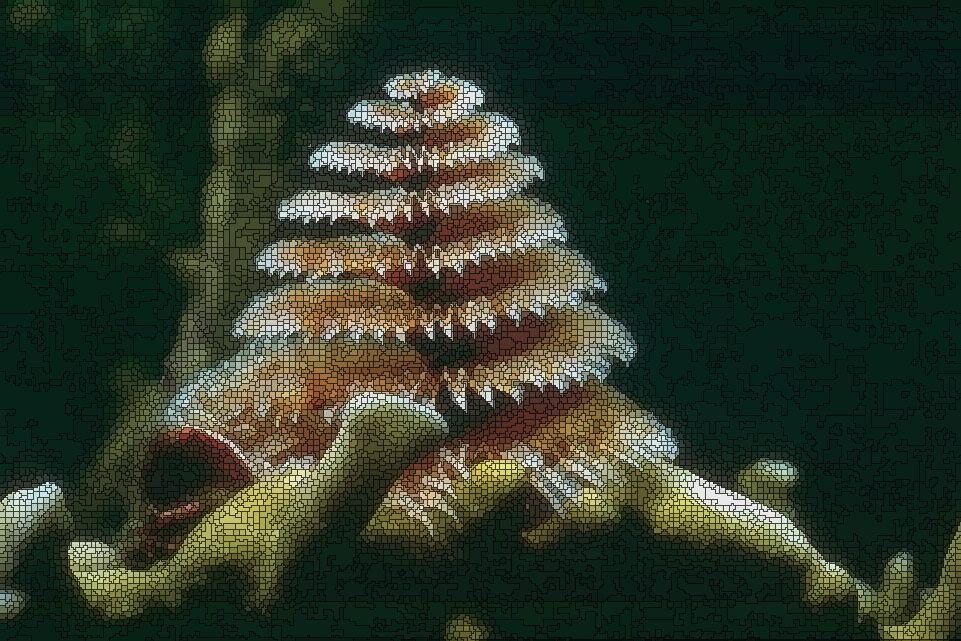
\includegraphics[width=4.82cm]{fig/12074/0.png}};
        \draw[black,very thick] (0,0) rectangle (4.81,3.21);
    \end{scope}

    \begin{scope}[yshift=60*1,every node/.append style={yslant=0.5,xslant=-1},yslant=0.5,xslant=-1]
        \draw[-latex,thick] (-0.17,3.21/2) node[right]{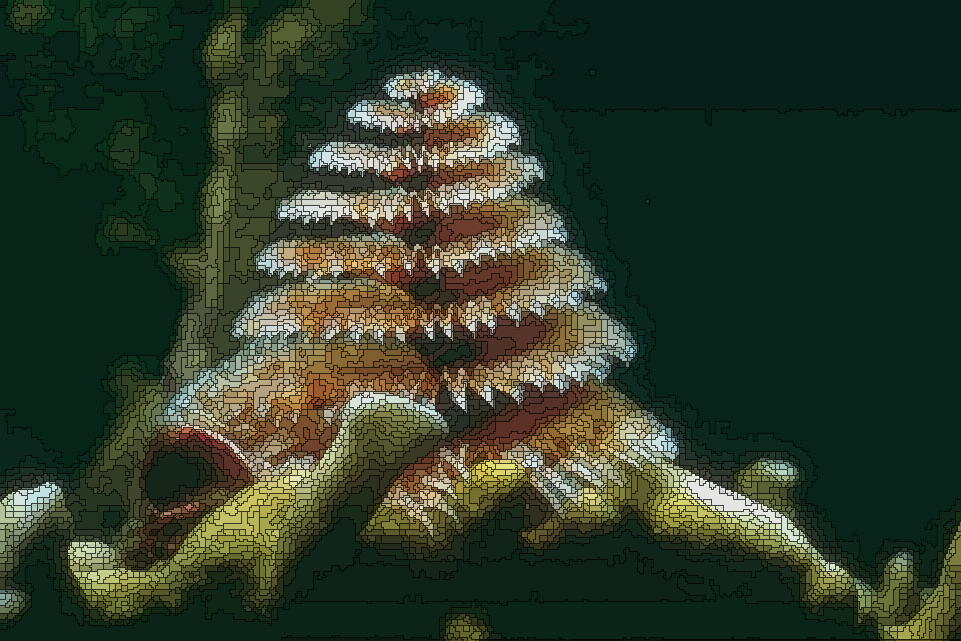
\includegraphics[width=4.82cm]{fig/12074/2.png}};
        \draw[black,very thick] (0,0) rectangle (4.81,3.21);
    \end{scope}

    \begin{scope}[yshift=60*2,every node/.append style={yslant=0.5,xslant=-1},yslant=0.5,xslant=-1]
        \draw[-latex,thick] (-0.17,3.21/2) node[right]{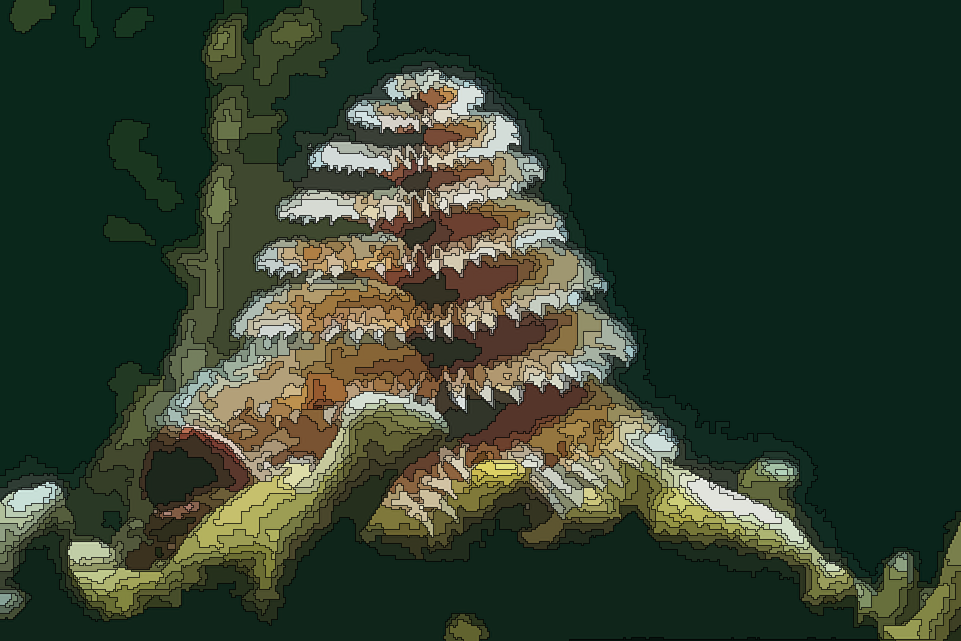
\includegraphics[width=4.82cm]{fig/12074/4.png}};
        \draw[black,very thick] (0,0) rectangle (4.81,3.21);
    \end{scope}

    \begin{scope}[yshift=60*3,every node/.append style={yslant=0.5,xslant=-1},yslant=0.5,xslant=-1]
        \draw[-latex,thick] (-0.17,3.21/2) node[right]{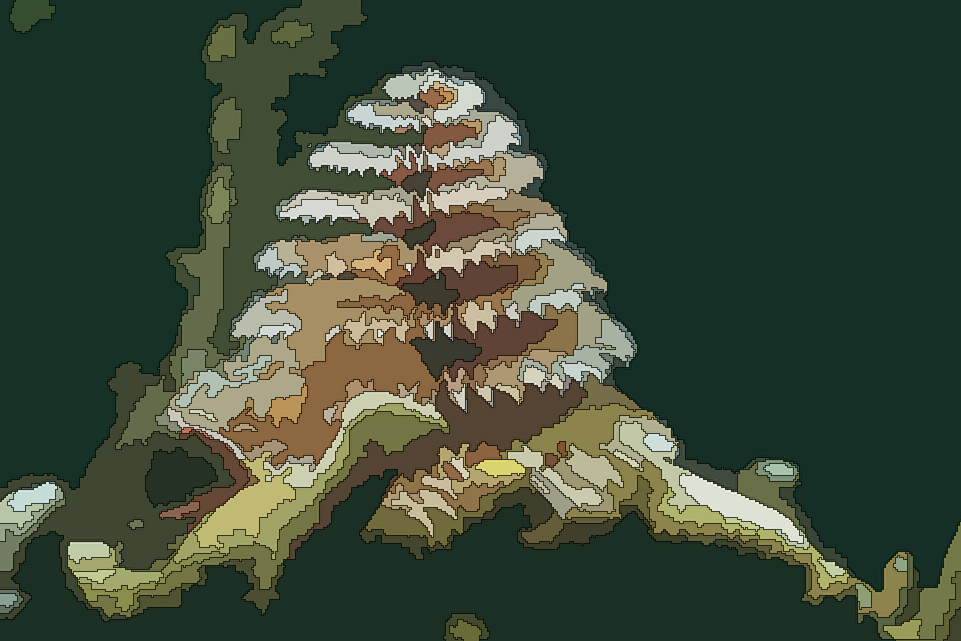
\includegraphics[width=4.82cm]{fig/12074/6.png}};
        \draw[black,very thick] (0,0) rectangle (4.81,3.21);
    \end{scope}

    \begin{scope}[yshift=60*4,every node/.append style={yslant=0.5,xslant=-1},yslant=0.5,xslant=-1]
        \draw[-latex,thick] (-0.17,3.21/2) node[right]{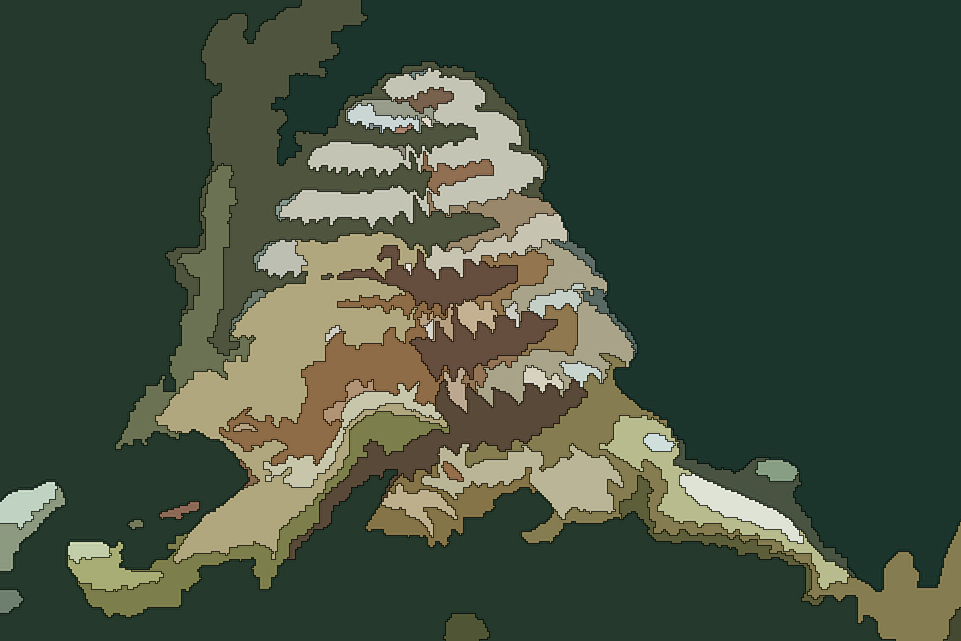
\includegraphics[width=4.82cm]{fig/12074/8.png}};
        \draw[black,very thick] (0,0) rectangle (4.81,3.21);
    \end{scope}


    \draw[->,-triangle 60] (-3,0) -- node[above]{time} (-3,4);

    %%%%%%%%%%%%%%%%%%%%%%%%%%%%%%%%%%%%%%%%%%%%%%%%%%%%%%%%%%%%%%%
    % 0 bottom layer
    %%%%%%%%%%%%%%%%%%%%%%%%%%%%%%%%%%%%%%%%%%%%%%%%%%%%%%%%%%%%%%%%
    \draw[-latex,thick] (6.2,2) node[right]{$\mathsf{over-segmentation}$}
         to[out=180,in=90] (4,2);
         
         
         
    %%%%%%%%%%%%%%%%%%%%%%%%%%%%%%%%%%%%%%%%%%%%%%%%%%%%%%%%%%%%%%%
    % 1 layer
    %%%%%%%%%%%%%%%%%%%%%%%%%%%%%%%%%%%%%%%%%%%%%%%%%%%%%%%%%%%%%%%%
    
    \draw[-latex,thick] (6.2,5.5) node[right]{$\mathsf{Region adjacency graph 1}$}
         to[out=180,in=90] (4,5.5);

\end{tikzpicture}






In this section we will explain the principles of graph based hierarchical clustering (HC),
and  give an overview of different methods which uses a graph based HC.
The main idea of HC is to build a hierarchy of nested clusters instead of
a single flat clustering.
Such a hierarchy of clusters can be visualized as a dendrogram (see \cref{fig:hc_bottom_up_top_down} ).
In general there are two different strategies for HC.
\begin{compactitem}
    \item Bottom-Up / Agglomerative HC (\cref{fig:hc_bottom_up}):

        Each node in the graph starts in its own cluster. 
        During the clustering pairs of adjacent nodes are merged 
        by contracting the edge between them.
        Not only the nodes can be merged but also the features associated with
        the nodes and the edges.
        The dendrogram / cluster-tree is grown from the leaf nodes (each node in the graph is a leaf)
        to the root (all nodes in a single cluster) 

    \item Top-Down HC (\cref{fig:hc_top_down}):

        All nodes start in one single cluster. Each cluster is recursively divided 
        into two or more clusters. 
        The dendrogram / cluster-tree is grown from the root  (all nodes in a single cluster)
        to the leafs (all nodes in a single cluster) 
\end{compactitem}



\begin{figure}[ht]
    \centering
    \subfloat[Bottom-Up: Nodes are merged with increasing time]{\label{fig:hc_bottom_up}
        {
            \begin{tikzpicture}[sloped]
                \node (a)    at (-6,0)      {a};
                \node (b)    at (-5,0)      {b};
                \node (c)    at (-4,0)    {c};
                \node (d)    at (-3,0)     {d};
                \node (e)    at (-2,0)       {e};

                \node (ab)   at (-5.5,1)    {};
                \node (cd)   at (-3.5,1)    {};
                \node (cde)  at (-2.75,2)       {};
                \node (all)  at (-4,3)    {};
                
                \node (root) at (-4,4) {root}; 

                \draw (a) |- (ab.center);
                \draw (b) |- (ab.center);
                \draw (c) |- (cd.center);
                \draw (d) |- (cd.center);
                \draw (e) |- (cde.center);
                \draw (cd.center) |- (cde.center);
                \draw (ab.center) |- (all.center);
                \draw (cde.center) |- (all.center);
                \draw (all.center) |- (root.center);

                \draw[->,-triangle 60] (-7,0) -- node[above]{time} (-7,4);
            \end{tikzpicture}
        }
    }\hspace{2cm}
    \subfloat[Top-Down: Nodes are divided with increasing time]{\label{fig:hc_top_down}
        {
            \begin{tikzpicture}[sloped]
                \node (a)    at (-6,0)      {a};
                \node (b)    at (-5,0)      {b};
                \node (c)    at (-4,0)    {c};
                \node (d)    at (-3,0)     {d};
                \node (e)    at (-2,0)       {e};

                \node (ab)   at (-5.5,1)    {};
                \node (de)   at (-2.5,1)    {};
                \node (cde)  at (-3.25,2)       {};
                \node (all)  at (-4,3)    {};
                
                \node (root) at (-4,4) {root}; 

                \draw (a) |- (ab.center);
                \draw (b) |- (ab.center);
                \draw (c) |- (cde.center);
                \draw (d) |- (de.center);
                \draw (e) |- (de.center);        
                \draw (de.center) |- (cde.center);
                \draw (ab.center) |- (all.center);
                \draw (cde.center) |- (all.center);
                \draw (all.center) |- (root.center);

                \draw [->,-triangle 60] (-7,4) -- node[below,align=center]{time} (-7,0);
            \end{tikzpicture}
        }
    }
    \caption{
        Describe the difference between both
    }
    \label{fig:hc_bottom_up_top_down}
\end{figure}



In this section we will only on bottom-up / agglomerative HC . 
In \cref{ch:cgc}  we propose an algorithm  based on top-down HC.

\subsection{Agglomerative Clustering}\label{sec:hc_agglomerative_clustering}

Agglomerative clustering benefits from the fact that noisy initial edge weights
become more informative due to the updating / merging of weights during the clustering.


\missingfigure{bla } \label{fig:hc_noise_reduction}


\subsubsection{Wards Methods}\label{sec:hc_wards_method}


\begin{equation} \label{eq:wards_method}
    d_{ward}(u,v) =  \frac{d(u,v)}{ \frac{1}{|u|} + \frac{1}{|v|} }
\end{equation}

\begin{equation} \label{eq:sqrt_wards_method}
    d_{\sqrt{\text{ward}}}(u,v) =  \frac{d(u,v)}{ \frac{1}{\sqrt{|u|}} + \frac{1}{\sqrt{|v|}} }
\end{equation}



\subsubsection{Ultrametric Contour Map}\label{sec:hc_ucm}

A generic framework for boundary extraction and image segmentation based
on bottom-up hierarchical clustering, named Ultrametric Contour Map (UCM), 
has been proposed by \citet{arbelaez_2006_cvpr} . 
Starting from an over-segmentation, a region adjacency graph (RAG) is set up.
The edges of the RAG are weighted by an edge indicator and therefore a measure  of dissimilarity.
The main idea of UCM is to iteratively contract the edge with the lowest weight, 
and updating the edge weights while doing so.

\section{MST Methods}\label{sec:rw_mst_methods}


